\documentclass[UTF8]{article}
\usepackage{graphicx}
\usepackage{subfigure}
\usepackage{amsmath}
\usepackage{makecell}
\usepackage[utf8]{inputenc}
\usepackage[space]{ctex} %中文包
\usepackage{listings} %放代码
\usepackage{xcolor} %代码着色宏包
\usepackage{CJK} %显示中文宏包
\usepackage{float}

\definecolor{mygreen}{rgb}{0,0.6,0}
\definecolor{mygray}{rgb}{0.5,0.5,0.5}
\definecolor{mymauve}{rgb}{0.58,0,0.82}
\lstset{
	backgroundcolor=\color{white}, 
	basicstyle = \footnotesize,       
	breakatwhitespace = false,        
	breaklines = true,                 
	captionpos = b,                    
	commentstyle = \color{mygreen}\bfseries,
	extendedchars = false,
	frame = shadowbox, 
	framerule=0.5pt,
	keepspaces=true,
	keywordstyle=\color{blue}\bfseries, % keyword style
	language = C++,                     % the language of code
	otherkeywords={string}, 
	numbers=left, 
	numbersep=5pt,
	numberstyle=\tiny\color{mygray},
	rulecolor=\color{black},         
	showspaces=false,  
	showstringspaces=false, 
	showtabs=false,    
	stepnumber=1,         
	stringstyle=\color{mymauve},        % string literal style
	tabsize=4,          
	title=\lstname           
}


%画图包
\usepackage{tikz}
%画图背景包
\usetikzlibrary{backgrounds}

%自定义命令
\newcommand{\psiG}{\psi_{G}}
%在tikz中画一个顶点
%#1:node名称
%#2:位置
%#3:标签
\newcommand{\newVertex}[3]{\node[circle, draw=black, line width=1pt, scale=0.8] (#1) at #2{#3}}
%在tikz中画一条边
\newcommand{\newEdge}[2]{\draw [black,very thick](#1)--(#2)}
%在tikz中放一个标签
%#1:名称
%#2:位置
%#3:标签内容
\newcommand{\newLabel}[3]{\node[line width=1pt] (#1) at #2{#3}}


\title{中国科学技术大学计算机学院\\《数据结构》报告}
\author{}
\date{}

\begin{document}
\maketitle
	\begin{figure}[H]
		\centering
		
\includegraphics[width=2.5in]{xiaohui.jpg}\vspace{0.5cm}\\
		\large{
			实验题目:栈、队列及其应用\\
			学生姓名:王章瀚\\
			学生学号:PB18111697\\
			完成日期:\today\\
		}\vspace{2cm}
		
		\large{计算机实验教学中心制\\2019年09月\\}
		\thispagestyle{empty}
		\clearpage  % 清除当页页码
	\end{figure}
	\newpage
	
	\section{实验要求}
	\subsection{概述}
	假设有一N×N的棋盘和N个皇后,请为这N个皇后进行布局使得这N个皇后互不攻击(即任意两个皇后
	不在同一行、同一列、同一对角线上)。\\
	\textbf{基本要求:}\\
	1. 输入N,输出N个皇后互不攻击的所有布局;\\
	2. 用非递归方法来解决N-皇后问题,即自己设置栈来处理。\\
	
	\subsection{输入与输出}
	输入棋盘大小(皇后数)N\par
	
	输出所有满足题目要求的棋盘。\par
	
	输入输出样例:\par
	\subsection{测试数据}
	\fbox{
		\parbox{0.8\linewidth}{
			Input:\\
			8\\
			utput:\\
			Q\#\#\#\#\#\#\#\\
			\#\#\#\#Q\#\#\#\\
			\#\#\#\#\#\#\#Q\\
			\#\#\#\#\#Q\#\#\\
			\#\#Q\#\#\#\#\#\\
			\#\#\#\#\#\#Q\#\\
			\#Q\#\#\#\#\#\#\\
			\#\#\#Q\#\#\#\#\\
			…… //所有布局方案\\
			92 //总布局数\\
		}
	}

	\section{设计思路}
	本实验的基本算法如下图所示:
	\begin{figure}[H]
		\centering
		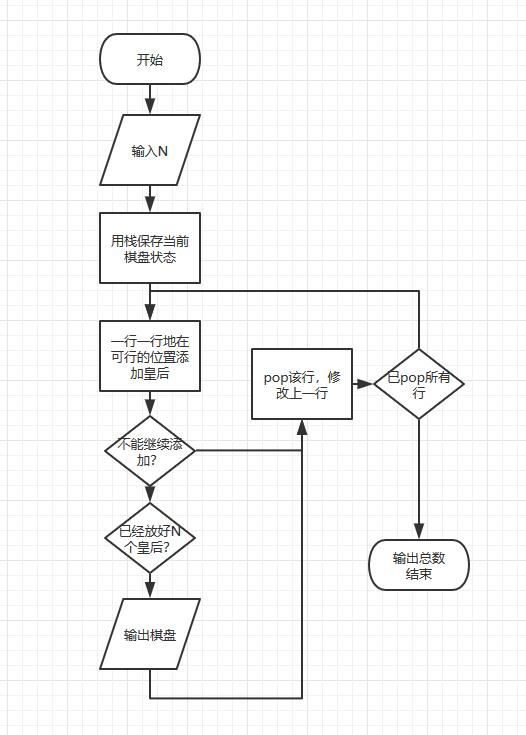
\includegraphics[scale=0.7]{algorithm.jpg}
		\caption{基本算法思路}
		\label{algorithm}
	\end{figure}\par

	本实验中,使用栈和递归来分别实现任务。\par
	其中,使用栈的方法时,定义了一个栈类型,后面会描述其定义。\par
	使用递归的方法则单纯使用一个线性表来存储当前正在处理的layout(布局)。\par
	而这两种方法的共同点是存储布局的方式——即使用一个N维线性表来存储每行放的皇后的列位置。\par
	
	
	\section{关键代码讲解}
	由于没有复杂的函数调用关系,故将函数调用关系图略去。\par
	且此处算法设计思路极其简单,即,逐行遍历layout的所有可能情况,如遇冲突,则撤销摆放,向前回溯,如遇成功,则输出,计数器自加。
	\subsection{栈}
	\subsubsection{数据类型的定义}
	1). 布局栈的定义
	\begin{lstlisting}[language=C++]
	// Here we use a stack to store the information of 
	// the layout.
	class layout {
	private:
		int cur;
		int size;
		int** layout_stack;
		
	public:
		layout(int N) {
			size = 0;
			cur = -1;
			this->N = N;
			layout_stack = new int*[N];
			for (int i = 0; i < N; i++) {
				layout_stack[i] = new int[N];
			}
		}
		
		int N;
		inline int stack_size() {
			return cur + 1;
		}
		
		int* top() {
			if (cur >= 0)
			return layout_stack[cur];
			return nullptr;
		}
		
		void pop() {
			if (cur >= 0) 
			delete layout_stack[cur--];
		}
		
		void push(int* cur_layout) {
			layout_stack[++cur] = cur_layout;
		}
		
		int* clone(int* ori);
		void printLayout(int* lay);
		bool is_lastline_ok(int* lay, int row);
		//use this function to solve the answer.
		void solve();
	};
	\end{lstlisting}
	
	\subsubsection{主要算法}
	主要算法即将流程图内容实现一遍,过程较为简单,详细说明已在下文注释:\par
	\begin{lstlisting}[language=C++]
	void solve() {
		clock_t start, end;
		start = clock();
		int counter = 0;
		int* cur_layout = new int[N];
		cur_layout[0] = 0;
		push(cur_layout);
		while (1) {
			cur_layout = clone(top());
			if (top() == nullptr)
				break;
			if (is_lastline_ok(cur_layout, stack_size() - 1)) {
				// no conflict here
				// whether finished
				if (stack_size() == N) {
					counter++;
					cout << counter << endl;
					printLayout(cur_layout);
				}
				else {
					cur_layout[stack_size()] = 0;
					push(cur_layout);
					continue;
				}
			}
			// need a recall
			delete[] cur_layout;
			cur_layout = top();
			if (cur_layout == nullptr)
				break;
			while (cur_layout[stack_size() - 1] == N - 1) {
				// tried all circumstance in this row
				pop();
				cur_layout = top();
				if (cur_layout == nullptr)
					break;
			}
			// found a row that the queen can be move rightward.
			if (cur_layout != nullptr) {
				top()[stack_size() - 1]++;
			}
		}
		end = clock();
		cout << "以上共" << counter << "种" << endl;
		cout << "耗时" << (double)(end - start) / CLOCKS_PER_SEC << "秒" << endl;
		
	}
	\end{lstlisting} 
	
	
	\subsection{递归}
	\subsubsection{主要算法}
	主要算法即将流程图内容实现一遍,过程较为简单,详细说明已在下文注释:\par
	\begin{lstlisting}[language=C++]
	// recursion method
	int counter = 0;
	void recursion(int* cur_layout, int row, const int N) {
		if (row == N) {
			counter++;
			// print the layout.
			cout << counter << endl;
			for (int i = 0; i < N; i++) {
				for (int j = 0; j < N; j++) {
					if (j == cur_layout[i]) cout << 'Q';
					else cout << '#';
				}
				cout << endl;
			}
			cout << endl;
			return;
		}
		for (int i = 0; i < N; i++) {
			cur_layout[row] = i;
			bool flag = true;
			// try all circumstances.
			for (int j = 0; j < row; j++) {
				if (cur_layout[j] == cur_layout[row] 
					|| abs(cur_layout[j] - cur_layout[row]) == row - j) {
					flag = false;
					break;
				}
			}
			// if ok, try next row. Here is the recursion.
			if(flag)
			recursion(cur_layout, row + 1, N);
		}
		return;
	}
	\end{lstlisting} 
	
	
	\section{调试分析}
	\subsection{问题发现与解决}
	在使用栈来保存布局时,由于指针的各种调用出现了一些混乱,经过Debug模式的观察,最终查出错误并解决。
	
	\subsection{算法的时空复杂度分析}
	由于遍历了几乎所有情况,而每行只需要尝试前面几行没有试过的,因此时间复杂度约为$o(n\times (n-1)\times \dots \times 1)=o(n!)$.\par
	下表展示了所用时间的表格。\\
	\begin{table}[H]
		\footnotesize
		\begin{tabular}{|c|c|c|c|c|c|c|c|c|c|}
			\hline 
			皇后数 & 4 & 5 & 6 & 7 & 8 & 9 & 10 & 11 & 12 \\ 
			\hline 
			栈/秒 & 0.0000736 & 0.0001495 & 0.0007673 & 0.0027767 & 0.0104837 & 0.048083 & 0.228105 & 1.2051 & 6.8581 \\ 
			\hline 
			递归/秒 & 0.0000035 & 0.0000092 & 0.0000458 & 0.0001814 & 0.0006057 & 0.0029883 & 0.0137117 & 0.0739021 & 0.421939 \\ 
			\hline 
		\end{tabular} 
	\end{table}
	下图红色是栈,蓝色是递归。灰色是用指数函数拟合的结果。\par
	\begin{figure}[H]
		\centering
		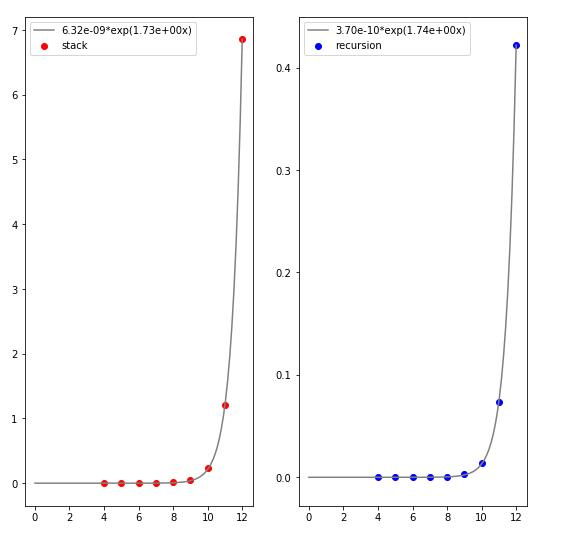
\includegraphics[scale=1]{time.jpg}
		\caption{time}
		\label{time}
	\end{figure}\par
	空间复杂度:对于栈方式,最多同时有$n$个大小为$n$的线性表存储所有布局,故为$o(n^{2})$.
	而对于递归,则只用了一个线性表存储,故为$o(n)$.\par
	
	\section{代码测试}
	\subsection{data1}
	\fbox{
		\parbox{0.8\linewidth}{
			Input:\\
			8\\
			Output:\\
			8\\
			栈解法:\\
			1\\
			Q\#\#\#\#\#\#\#\\
			\#\#\#\#Q\#\#\#\\
			\#\#\#\#\#\#\#Q\\
			\#\#\#\#\#Q\#\#\\
			\#\#Q\#\#\#\#\#\\
			\#\#\#\#\#\#Q\#\\
			\#Q\#\#\#\#\#\#\\
			\#\#\#Q\#\#\#\#\\
			...\\
			92\\
			以上共92种\\
			耗时0.842秒\\
			\\
			递归解法:\\
			1\\
			Q\#\#\#\#\#\#\#\\
			\#\#\#\#Q\#\#\#\\
			\#\#\#\#\#\#\#Q\\
			\#\#\#\#\#Q\#\#\\
			\#\#Q\#\#\#\#\#\\
			\#\#\#\#\#\#Q\#\\
			\#Q\#\#\#\#\#\#\\
			\#\#\#Q\#\#\#\#\\
			...\\
			92\\
			以上共92种\\
			耗时0.965秒\\
		}
	}\\
	截图如下:
	\begin{figure}[H]
		\centering
		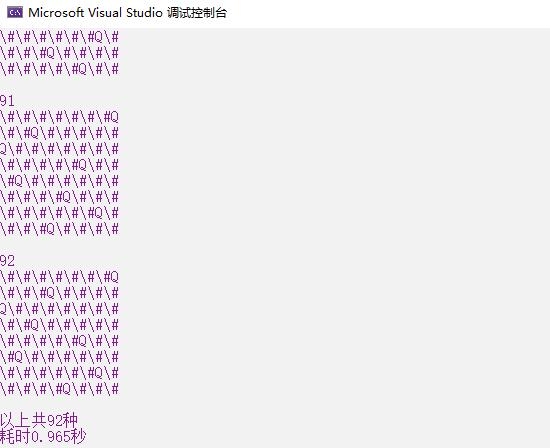
\includegraphics[scale=0.7]{data1.jpg}
		\caption{data1}
		\label{data1}
	\end{figure}\par
	
	\subsection{data2}
	\fbox{
		\parbox{0.8\linewidth}{
			Input:\\
			4\\
			Output:\\
			4\\
			栈解法:\\
			1\\
			\#Q\#\#\\
			\#\#\#Q\\
			Q\#\#\#\\
			\#\#Q\#\\
			\\
			2\\
			\#\#Q\#\\
			Q\#\#\#\\
			\#\#\#Q\\
			\#Q\#\#\\
			\\
			以上共2种\\
			耗时0.003秒\\
			\\
			递归解法:\\
			1\\
			\#Q\#\#\\
			\#\#\#Q\\
			Q\#\#\#\\
			\#\#Q\#\\
			\\
			2\\
			\#\#Q\#\\
			Q\#\#\#\\
			\#\#\#Q\\
			\#Q\#\#\\
			\\
			以上共2种\\
			耗时0.002秒\\
		}
	}\\
	截图如下:
	\begin{figure}[H]
		\centering
		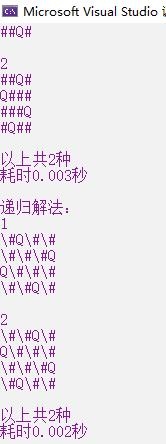
\includegraphics[scale=0.7]{data2.jpg}
		\caption{data2}
		\label{data2}
	\end{figure}\par


	\section{实验总结}
	通过本次的实验,本人更加熟悉了栈的使用。理解了怎么将一个递归的程序用栈来表示。\par
	但由于算法原因,N不能过大。尝试使用fork/join,N=16时依然需要一分多钟。\par


	\begin{figure}[H]
		\centering
		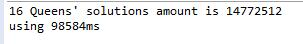
\includegraphics[scale=0.7]{concurrent.jpg}
		\caption{concurrent}
		\label{concurrent}
	\end{figure}\par



	\section{附录}
	\subsection{N皇后问题}
	\begin{lstlisting}[language=C++]
	#include <iostream>
	#include <cmath>
	#include <ctime>
	#include <windows.h>
	using namespace std;
	
	
	// Here we use a stack to store the information of 
	// the layout.
	class layout {
	private:
		int cur;
		int size;
		int** layout_stack;
		
	public:
		layout(int N) {
			size = 0;
			cur = -1;
			this->N = N;
			layout_stack = new int*[N];
			for (int i = 0; i < N; i++) {
				layout_stack[i] = new int[N];
			}
		}
		
		int N;
		inline int stack_size() {
		return cur + 1;
		}
		
		// get the top of stack
		int* top() {
			if (cur >= 0)
				return layout_stack[cur];
			return nullptr;
		}
		
		// pop the top of the stack
		void pop() {
			if (cur >= 0) 
				delete layout_stack[cur--];
		}
		
		// push cur_layout to the top of the stack
		void push(int* cur_layout) {
			layout_stack[++cur] = cur_layout;
		}
		
		// clone a layout and return it.
		int* clone(int* ori) {
			if (ori == nullptr)
				return nullptr;
			auto temp = new int[N];
			for (int i = 0; i < N; i++) {
				temp[i] = ori[i];
			}
			return temp;
		}
		
		// print the layout.
		void printLayout(int* lay) {
			for (int i = 0; i < N; i++) {
				for (int j = 0; j < N; j++) {
					if (j == lay[i]) cout << 'Q';
					else cout << '#';
				}
				cout << endl;
			}
			cout << endl;
		}
		
		// to determine whether the last line in lay is ok.
		bool is_lastline_ok(int* lay, int row) {
			for (int j = 0; j < row; j++) {
				if (lay[j] == lay[row] || abs(lay[j] - lay[row]) == row - j) {
					return false;
				}
			}
			return true;
		}
		
		void solve() {
			LARGE_INTEGER start, nFreq, end;
			QueryPerformanceFrequency(&nFreq);
			QueryPerformanceCounter(&start);
			int counter = 0;
			int* cur_layout = new int[N];
			cur_layout[0] = 0;
			push(cur_layout);
			while (1) {
				cur_layout = clone(top());
				if (top() == nullptr)
					break;
				if (is_lastline_ok(cur_layout, stack_size() - 1)) {
					// no conflict here
					// whether finished
					if (stack_size() == N) {
						counter++;
						cout << counter << endl;
						printLayout(cur_layout);
					}
					else {
						cur_layout[stack_size()] = 0;
						push(cur_layout);
						continue;
					}
				}
				// need a recall
				delete[] cur_layout;
				cur_layout = top();
				if (cur_layout == nullptr)
					break;
				while (cur_layout[stack_size() - 1] == N - 1) {
					// tried all circumstance in this row
					pop();
					cur_layout = top();
					if (cur_layout == nullptr)
						break;
				}
				// found a row that the queen can be move rightward.
				if (cur_layout != nullptr) {
					top()[stack_size() - 1]++;
				}
			}
			QueryPerformanceCounter(&end);
			cout << "以上共" << counter << "种" << endl;
			cout << "耗时" << (double)(end.QuadPart - start.QuadPart) / (double)nFreq.QuadPart << "秒" << endl;
			
		}
	
	};
	
	
	// recursion method
	int counter = 0;
	void recursion(int* cur_layout, int row, const int N) {
	if (row == N) {
	counter++;
	// print the layout.
	cout << counter << endl;
	for (int i = 0; i < N; i++) {
	for (int j = 0; j < N; j++) {
	if (j == cur_layout[i]) cout << 'Q';
	else cout << "#";
	}
	cout << endl;
	}
	cout << endl;
	return;
	}
	for (int i = 0; i < N; i++) {
	cur_layout[row] = i;
	bool flag = true;
	// try all circumstances.
	for (int j = 0; j < row; j++) {
	if (cur_layout[j] == cur_layout[row] 
	|| abs(cur_layout[j] - cur_layout[row]) == row - j) {
	flag = false;
	break;
	}
	}
	// if ok, try next row. Here is the recursion.
	if(flag)
	recursion(cur_layout, row + 1, N);
	}
	return;
	}
	
	
	int main()
	{
		int N;
		cin >> N;
		
		cout << "栈解法:\n";
		layout lay(N);
		lay.solve();
		
		cout << "\n递归解法:\n";
		int* cur_layout = new int[N];
		LARGE_INTEGER start, nFreq, end;
		QueryPerformanceFrequency(&nFreq);
		QueryPerformanceCounter(&start);
		recursion(cur_layout, 0, N);
		QueryPerformanceCounter(&end);
		cout << "以上共" << counter << "种" << endl;
		cout << "耗时" << (double)(end.QuadPart - start.QuadPart) / (double)nFreq.QuadPart << "秒" << endl;
	}
	
	\end{lstlisting}

\end{document}
